% =========================================================================== %

\begin{frame}[t,plain]
\titlepage
\end{frame}

% =========================================================================== %

\begin{frame}{Recap}
%
\begin{columns}[T]
\column{.5\linewidth}
\texttt{pd.Series}
\begin{itemize}
\item Represents One Column of Data
\item Built on NumPy Arrays
\item Arbitrary Indices
\item Element-Wise Operations
\item Index Alignment
\item Reduction Functions
\item Boolean Array Indexing
\end{itemize}
%
\column{.5\linewidth}
\texttt{pd.DataFrame}
\begin{itemize}
\item Represents a Table of Data
\item Collection of \texttt{pd.Series}
\item Reader and Writer for Many Standard Formats
\item Non-Owning Views
\item Grouping, Binning and Sorting
\item Iterating over Data
\item Connection to MatPlotLib
\end{itemize}

\end{columns}
%
\begin{center}
	\emph{Any Questions?}
\end{center}
%
\end{frame}

% =========================================================================== %

\begin{frame}{Old Files}
%
\begin{columns}[T]
\column{.22\linewidth}
\includegraphics[width=\linewidth]{./gfx/xkcd-oldfiles}
%
\column{.5\linewidth}
\begin{center}
\emph{Wow, ANIMORPHS-NOVEL.RTF? Just gonna, uh, go through and delete that from all my archives real quick.}

\vspace{12pt}
Source: \url{https://xkcd.com/1360/}
\end{center}
\end{columns}
%
\end{frame}

% =========================================================================== %

\begin{frame}
%
\begin{center}
	\includegraphics[width=.9\linewidth, page=1]{./gfx/filesystems}
\end{center}
%
\end{frame}

% =========================================================================== %

\begin{frame}{Structure Elements of a Partition}
%
\begin{columns}
\column{.7\linewidth}
	\includegraphics[width=\linewidth, page=2]{./gfx/filesystems}
%
\column{.3\linewidth}
	\small
	\begin{itemize}
	\item There can be multiple file systems (partitions) on a single physical device.
	\item There are dozens of file systems, all with their particular inner workings
	\item The scheme holds for most common file systems, such as NTFS, ext or hfs+
	\item We could do an entire lecture \emph{series} on file systems alone
	\end{itemize}
\end{columns}
%
\end{frame}

% =========================================================================== %

\begin{frame}{Regular Files and Fragmentation}
%
% trim = left bottom right top
\includegraphics[width=\linewidth, page=3,trim=0 300 0 20,clip]{./gfx/filesystems}
%
\begin{columns}
\column{.5\linewidth}
	\begin{itemize}
	\item List of entries: tuples of strings and inodes
	\item Inodes: Metadata and actual location: block ID
	\end{itemize}
%
\column{.5\linewidth}
	\begin{itemize}
	\item Blocks: fixed size
	\item Larger files: multiple blocks
	\item[\Thus] Fragmentation
	\end{itemize}
\end{columns}
%
\end{frame}

% =========================================================================== %

\begin{frame}{Hardlinks}
%
% trim = left bottom right top
\includegraphics[width=\linewidth, page=4,trim=0 300 0 20,clip]{./gfx/filesystems}
%
\begin{columns}
\column{.5\linewidth}
	\begin{itemize}
	\item Multiple entries in List of Entries can point to same inode
	\item[\Thus] Same file in two (or more) locations
	\item Changes affect both locations
	\end{itemize}
%
\column{.5\linewidth}
	\begin{itemize}
	\item Imagine shared ressource for several project folders
	\item File is only deleted when all references are removed
	\end{itemize}
\end{columns}
%
\end{frame}

% =========================================================================== %

\begin{frame}{Symbolic Links (aka SymLinks)}
%
% trim = left bottom right top
\includegraphics[width=\linewidth, page=5,trim=0 300 0 20,clip]{./gfx/filesystems}
%
\begin{columns}
\column{.5\linewidth}
	\begin{itemize}
	\item Speical kind of inode
	\item Content: referenced file
	\item In principle same effect
	\end{itemize}
%
\column{.5\linewidth}
	\begin{itemize}
	\item Moving/Deleting original file breaks link
	\item Works with folders and across file systems
	\end{itemize}
\end{columns}
%
\end{frame}

% =========================================================================== %

\begin{frame}{Link Files}
%
% trim = left bottom right top
\includegraphics[width=\linewidth, page=6,trim=0 300 0 20,clip]{./gfx/filesystems}
%
\begin{columns}
\column{.5\linewidth}
	\begin{itemize}
	\item Like SymLinks, but done in regular files
	\item Treated by GUI rather than OS
	\item Same (dis)advantages
	\end{itemize}
%
\column{.5\linewidth}
	\begin{itemize}
	\item Windows: \texttt{.lnk} files
	\item Linux: \texttt{.desktop} files
	\item Mac: I don't have a fucking clue
	\end{itemize}
\end{columns}
%
\end{frame}

% =========================================================================== %

\begin{frame}
%
\begin{columns}
\column{.5\linewidth}
\begin{hintbox}[Following Symlinks and Link Files]
	Not all programs automatically follow symlinks. \emph{Most} programs don't follow link files. One example is a zip program I was using two years ago, to the effect
	that I nearly failed a course.\\
	
	You can find out about the nature by visual clues: in Windows, link files and symlinks are rendered with an arrow in the lower left corner.
	Depending on your file browser, symlinks sometimes are rendered in different colours.\\
	
	In the console, \texttt{ls -l} (Linux/Mac) or \texttt{dir /a} (Windows) reveals the true nature of a file.
\end{hintbox}
%
\column{.5\linewidth}
	\begin{center}
		
\includegraphics[width=.4\linewidth]{./gfx/link-folder}
	\end{center}
	
	\begin{center}
		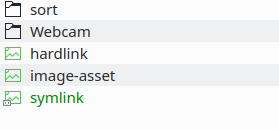
\includegraphics[width=.8\linewidth]{./gfx/link-linux}
	\end{center}
	
	\begin{center}
		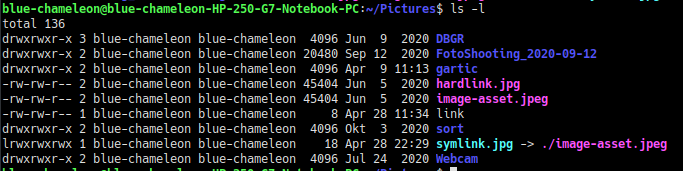
\includegraphics[width=1.\linewidth]{./gfx/link-konsole}
	\end{center}
	
	
\end{columns}
%
\end{frame}

% =========================================================================== %

\begin{frame}{Todays Modules}
%
\begin{itemize}
\item \texttt{os} -- Operating System Functions
	\begin{itemize}
	\item Common interface to OS-specific calls
	\item Mostly: deal with the file system
	\item \url{https://docs.python.org/3/library/os.html}
	\item Submodule \texttt{path}
	\item \url{https://docs.python.org/3/library/os.path.html}
	\end{itemize}
\item \texttt{glob} -- Frontend for \texttt{os}
	\begin{itemize}
	\item Easy traversal of folder structures
	\item \url{https://docs.python.org/3/library/glob.html}
	\end{itemize}
\item \texttt{sys} -- Python Interna
	\begin{itemize}
	\item Command line parameters
	\item Memory model
	\item Default behaviour
	\item \url{https://docs.python.org/3/library/sys.html}
	\end{itemize}
\end{itemize}
%
\end{frame}

% =========================================================================== %

\begin{frame}{Controlling Directories}
%
\begin{itemize}
\item \texttt{os.chdir(path)} -- change CWD to \texttt{path}, given as string
\item \texttt{os.getcwd()} -- find out CWD as string
\item \texttt{os.curdir} and \texttt{os.pardir} -- string constants \inPy{'.'} and \inPy{'..'}
\item \texttt{os.mkdir(subfolder)} -- create \texttt{subfolder} under the CWD, where subfolder is a string
\item \inPy{os.makedirs("multiple/subdirs/at/once")}
\item \texttt{os.rmdir(directory)} -- delete \emph{empty} directory, given as string
	\begin{itemize}
	\item May neither contain files nor subdirectories
	\item Otherwise raises \texttt{OSError: [Errno 39] Directory not empty: 'directory'}
	\end{itemize}
\end{itemize}
%
\end{frame}

% =========================================================================== %

\begin{frame}{Controlling Files}
%
\begin{itemize}
\item \texttt{os.remove(filename)} -- delete a file
\item \texttt{os.rename(src, dst)} -- change filename or move a file
	\begin{itemize}
	\item E.\;g.: \inPy{os.rename("./sourceDir/file", "./destinationDir/newName")}
	\end{itemize}
\item \texttt{os.link(source, link)} -- creates a hardlink from \texttt{sorce} with name \texttt{link}, both strings
\item \texttt{os.symlink(source, link)} -- creates a hardlink from \texttt{sorce} with name \texttt{link}, both strings
\item Remember: Create files with Python's \inPy{open} command
\end{itemize}
%
\end{frame}

% =========================================================================== %

\begin{frame}[fragile]{Traversing the File System}
%
\begin{itemize}
\item \inPy{os.listdir(path='.')}
	\begin{itemize}
	\item Returns a \inPy{list} of strings
	\item All elements in the CWD
	\item Regardless of type (file, symlink, directory)
	\item Does not contain \inPy{'.'} and \inPy{'..'}
	\end{itemize}
\item \inPy{os.scandir(path='.')}
	\begin{itemize}
	\item Returns iterator to \texttt{os.Direntry} object (see next slide)
	\item Object has \inPy{__enter__} and \inPy{__exit__}, \ie is compatible with \inPy{with}:\\
\begin{minted}{python3}
with os.scandir() as it :
    for entry in it :
        commands
\end{minted}
	\end{itemize}
\item For both of them
	\begin{itemize}
	\item No particular order
	\item Neither of them supports wildcards (\texttt{*} or \texttt{?} -- see later)
	\end{itemize}
\end{itemize}
%
\end{frame}

% =========================================================================== %

\begin{frame}{Traversing the File System: The \texttt{Direntry} Object}
%
\inPy{it = os.scandir()}
\begin{itemize}
\item Iterator -- \inPy{for entry in it:} or \inPy{entry = next(it)}
\item \inPy{entry.name} -- file name as string, relative to path in \texttt{scandir}
\item \inPy{entry.path} -- full file name, including path, as string
\item \inPy{entry.is_dir()}, \inPy{entry.file()}, \inPy{entry.symlink()} -- booleans, identifying the kind of entry
\item \inPy{entry.file(follow_symlinks=True)}
	\begin{itemize}
	\item If \inPy{follow_symlinks=True}: returns \inPy{True} only if symlink is not broken
	\item Otherwise: Returns \inPy{False} when encountering a symlink
	\end{itemize}
\item \texttt{it.close()}
	\begin{itemize}
	\item Ends iteration, frees ressources
	\item Not needed when used in \inPy{with} block
	\item \enquote{Only} slows down OS when forgotten
	\end{itemize}
\end{itemize}
%
\end{frame}

% =========================================================================== %

\begin{frame}[fragile]
%
\begin{tcbraster}[raster columns=2,
                  raster equal height,
                  nobeforeafter,
                  raster column skip=0.5cm]
\begin{codebox}[Example: \texttt{listdir}]
\begin{minted}[linenos, fontsize=\scriptsize]{python3}
import os


for entry in os.listdir() :
    print(entry)
\end{minted}
\end{codebox}
%
\begin{codebox}[Example: \texttt{scandir}]
\begin{minted}[linenos, fontsize=\scriptsize]{python3}
import os

with os.scandir() as it :
    for entry in it :
        print(entry)
        \end{minted}
\end{codebox}
\end{tcbraster}
%
\begin{tcbraster}[raster columns=2,
                  raster equal height,
                  nobeforeafter,
                  raster column skip=0.5cm]
\begin{cmdbox}[Output: \texttt{listdir}]
\begin{minted}[fontsize=\scriptsize]{text}
Erstiheft
schausche.jpg
stuff01
civ3-ptw-manual.pdf
RBS.txt
.directory
stuff2
stuff1
PK_Strunk_Exp_Mechanik.pdf
\end{minted}
\end{cmdbox}
%
\begin{cmdbox}[Output: \texttt{scandir}]
\begin{minted}[fontsize=\scriptsize]{text}
<DirEntry 'Erstiheft'>
<DirEntry 'schausche.jpg'>
<DirEntry 'stuff01'>
<DirEntry 'civ3-ptw-manual.pdf'>
<DirEntry 'RBS.txt'>
<DirEntry '.directory'>
<DirEntry 'stuff2'>
<DirEntry 'stuff1'>
<DirEntry 'PK_Strunk_Exp_Mechanik.pdf'>
\end{minted}
\end{cmdbox}
\end{tcbraster}
%
\end{frame}

% =========================================================================== %

\begin{frame}[fragile]{Traversing the File System: \texttt{glob} Module}
%
\begin{itemize}
\item Often: Need to filter for a certain file type (\eg \texttt{.jpg} files)
\item Or: Need to traverse \emph{recursively} (subfolders of subfolders of ...)
\item \inPy{glob.glob(path, recursive=False)}
	\begin{itemize}
	\item Return a (possibly empty) \inPy{list} of strings
	\item Relative to \texttt{path}
	\item May contain \emph{Wildcards} (see next slide)
	\item If \inPy{recursive=True}, subfolders are explored, too
	\item Broken symlinks are included
	\end{itemize}
\end{itemize}
%
\begin{hintbox}[Module \texttt{pathlib} and \texttt{os.walk}]
\small
Pythons \texttt{pathlib} offes an object oriented approach to file system travesal. It is built upon \texttt{os} and \texttt{glob}, but a little more unwieldy for most cases. Go have a look at it under \url{https://docs.python.org/3/library/pathlib.html}.

Finally, have a look at \texttt{os.walk} which allows to explore a directory tree conveniently.\\
See \url{https://docs.python.org/3/library/os.html#os.walk}
\end{hintbox}
%
\end{frame}

% =========================================================================== %

\begin{frame}{Wildcards}
%
\begin{itemize}
\item Like escape characters -- stand in characters
\item \texttt{?} -- an arbitrary character
	\begin{itemize}
	\item E.\;g. \texttt{myFile-?.ext} matches \texttt{myFile-a.ext}, \texttt{myFile-A.ext}, \texttt{myFile-0.ext}, ... but not \texttt{myFile-aa.ext} or
	\texttt{myFile-.ext}
	\end{itemize}
\item \texttt{*} -- any number of arbitrary characters
	\begin{itemize}
	\item E.\;g. \texttt{*.jpg} matches \emph{all} \texttt{jpg} files
	\item E.\;g. \texttt{a*.ext} matches \texttt{abcde.ext} and even \texttt{a.ext}
	\end{itemize}
\item \texttt{**} -- any number of subdirectories (including zero)
	\begin{itemize}
	\item Only when \inPy{recursive = True}
	\end{itemize}
\item \texttt{[wildcard]} -- literal matching
\end{itemize}
%
\begin{hintbox}[Rules for Filenames]
If your filenames contain ?, *, <, |, >, [, ], /, \, " or \$, you're using your computer wrong.
\end{hintbox}
%
\end{frame}

% =========================================================================== %

\begin{frame}[fragile]
%
\begin{codebox}[Example: Traversal]
\begin{minted}[linenos, fontsize=\scriptsize]{python3}
import glob

print( glob.glob("**") )
print( glob.glob("**/*.tex", recursive=True) )
\end{minted}
\end{codebox}
%
\begin{cmdbox}[Output: Traversal]
\begin{minted}[fontsize=\scriptsize]{text}
['02-codes', 'Install-Lines', '00-blurb', '04-vids', 'sebi-notes', 'gesina-notes',
 'unicode-fail.png', '01-tex', 'notepad-plus-utf8.png', 'tree.py', '03-exos']
['01-tex/03_main_decorators.tex', '01-tex/02_main_iterators.tex', '01-tex/01_content.tex',
 '01-tex/05_content.tex', '01-tex/01_main_efficiency.tex', '01-tex/04_content.tex',
 '01-tex/07_content.tex', '01-tex/06_content.tex', '01-tex/02_content.tex',
 '01-tex/04_main_SciPy.tex', '01-tex/05_main_tkInter.tex', '01-tex/06_main_pandas.tex',
 '01-tex/07_main_ossysglob.tex', '01-tex/03_content.tex',
 '01-tex/99_content-template.tex', '03-exos/X03/03-problems.tex',
 '03-exos/X04/04-problems.tex', '03-exos/X06/06-problems.tex',
 '03-exos/X02/02-problems.tex', '03-exos/X01/01-problems.tex',
 '03-exos/X05/05-problems.tex']
\end{minted}
\end{cmdbox}
%
\end{frame}

% =========================================================================== %

\begin{frame}{Path Utility Module -- \texttt{os.path}}
%
\begin{itemize}
\item \texttt{os.path.abspath(path)} -- get the absolute path from a location relative to the CWD
	\begin{itemize}
	\item \inPy{"someString" } gives \inPy{"/absolute/path/to/someString"}
	\item \inPy{"/someString"} gives \inPy{"/someString"}
	\end{itemize}
\item \texttt{os.path.join(pathA, pathB)} -- concatenates strings and makes sure slashes are joint correctly
	\begin{itemize}
	\item \inPy{"A" , "B"} gives \inPy{"A/B"}
	\item \inPy{"A/", "B"} gives \inPy{"A/B"}
	\item \inPy{"A", "/B"} gives \inPy{"/B"}
	\end{itemize}
\item \texttt{os.path.split(path)} -- splits \texttt{path} into \texttt{[directory, filename]}
	\begin{itemize}
	\item \inPy{"root/directory/someFile"} gives \inPy{["root/directory", "someFile"]}
	\item \inPy{"root/directory/someFile/"} gives \inPy{["root/directory/someFile", ""]}
	\item \inPy{"someFile"} gives \inPy{["", "someFile"]}
	\item Note: no check whether \texttt{someFile} is actually a file!
	\end{itemize}
\end{itemize}
%
\end{frame}

% =========================================================================== %

\begin{frame}{Path Utility Module -- \texttt{os.path}}
%
\begin{itemize}
\item \texttt{os.path.exists(path)} \texttt{os.path.lexists(path)}
	\begin{itemize}
	\item Both return \inPy{True} if \texttt{path} specifies an existing file
	\item Follows SymLinks
	\item \texttt{lexists} also returns \inPy{True} for \emph{broken} SymLinks
	\end{itemize}
\item \texttt{os.path.getsize(path)}
	\begin{itemize}
	\item Returns size of file in bytes
	\item Raises an \inPy{OSError} if the file does not exist or is inaccessible.
	\end{itemize}
\item \texttt{os.path.isfile(path)}, \texttt{os.path.isdir(path)}, \texttt{os.path.islink(path)}
	\begin{itemize}
	\item Like the methods of \texttt{os.DirEntry}
	\end{itemize}
\item \texttt{os.path.samefile(pathA, pathB)}
	\begin{itemize}
	\item Returns \inPy{True} if \texttt{pathA} and \texttt{pathB} specify the same file
	\item Follows SymLinks
	\item Uses Inode to do its job (\ie same content will not return \inPy{True})
	\end{itemize}
\end{itemize}
%
\end{frame}

% =========================================================================== %

\begin{frame}{Command Line Options}
%
\begin{itemize}
\item Recap: You can start your Python codes from the command line:\\
	\texttt{python3 yourCode.py}
\item Further command line options for the Python interpreter: \url{https://docs.python.org/3/using/cmdline.html}
\item Script (or module) must be the last command line argument
\item \texttt{sys.argv}
	\begin{itemize}
	\item Returns a \inPy{list} of all command line arguments
	\item Includig the Code file
	\item Excluding the interpreter invocation
	\item Excluding interpreter parameters
	\end{itemize}
\end{itemize}
%
\end{frame}

% =========================================================================== %

\begin{frame}
%
\begin{hintbox}[Shebang Mechanism for Linux and Mac]
\small
Text files beginning with \texttt{\#!} (called a \emph{shebang}) followed by an absolute path to an interpreter and with the executable flag set can be invoked from the source file alone.

Begin your files with \texttt{\#!/usr/bin/python3} and start them from console like a regular command
\end{hintbox}
%
\begin{hintbox}[File Associations under Windows]
\small
Under Windows, how a file is interpreted is determined by its extension. The \emph{Windows Registry} is a collection of system wide settings that, among other things, tells the system which filetypes to open with which programs. The key\\
\texttt{[HKEY\_CLASSES\_ROOT\textbackslash py\_auto\_file\textbackslash shell\textbackslash Open\textbackslash command]}\\
can be edited to change the associations with the file type.

\vspace{3pt}
Warning: Only edit the registry if you really know what you're doing.\\
In doubt, keep typing \texttt{python myCode.py}.

\vspace{3pt}
\scriptsize
\url{https://www.computerhope.com/issues/ch001348.htm}\\
\url{https://superuser.com/questions/669142/how-to-set-file-association-in-windows-explorer}
\end{hintbox}
%
\end{frame}

% =========================================================================== %

\begin{frame}[fragile]
%
\begin{codebox}[Example: \texttt{shebang.py}]
\begin{minted}[linenos, fontsize=\scriptsize]{python3}
#!/usr/bin/python3
import sys
print(sys.argv)
\end{minted}
\end{codebox}
%
\begin{cmdbox}[Console: \texttt{shebang.py}]
\scriptsize
{\color{green}blue-chameleon@blue-chameleon-HP-250-G7-Notebook-PC}:{\color{blue}\textasciitilde/tmp}\$
./shebang.py

['./shebang.py']

{\color{green}blue-chameleon@blue-chameleon-HP-250-G7-Notebook-PC}:{\color{blue}\textasciitilde/tmp}\$
./shebang.py bla ble "and more"

['./shebang.py', 'bla', 'ble', 'and more']

{\color{green}blue-chameleon@blue-chameleon-HP-250-G7-Notebook-PC}:{\color{blue}\textasciitilde/tmp}\$
./shebang.py options

['./shebang.py', 'options']

{\color{green}blue-chameleon@blue-chameleon-HP-250-G7-Notebook-PC}:{\color{blue}\textasciitilde/tmp}\$
python3 -I ./shebang.py options

['./shebang.py', 'options']
\end{cmdbox}
%
\end{frame}

% =========================================================================== %

\begin{frame}{Pipes and Device Files: stdin, stdout, stderr}
%
\begin{itemize}
\item Output to / Input from the console: formally writing/reading a \emph{file}
\item Same OS infrastructure like files (\eg buffers), but ultimatively different hardware
\item \texttt{sys.stdin} -- standard input: where \inPy{input} takes its results from
\item \texttt{sys.stdout} -- standard output: where \inPy{print} writes to
\item \texttt{sys.stderr} -- usually the same as stdout. Used for error messages
\item Can be \emph{redirected}
	\begin{itemize}
	\item \texttt{command > file}: send data written to stdout in \texttt{file} (overwrite)
	\item \texttt{command >{}> file}: append to \texttt{file} instead of overwriting
	\item \texttt{command 2> file} and \texttt{command 2>{}> file}: same for stderr
	\item \texttt{command 2>\&1}: redirect stderr to stdout
	\item \texttt{command > file 2>\&1}: redirect both, stdout and stderr to \texttt{file}
	\item \texttt{command < file}: use file as input for \texttt{command}
	\item \texttt{cmdA | cmdB}: use output (stdout) of \texttt{cmdA} as input for \texttt{cmdB}
	\end{itemize}
\end{itemize}
%
\end{frame}

% =========================================================================== %

\begin{frame}[fragile]
%
\begin{codebox}[Example: \texttt{channels.py}]
\begin{minted}[linenos, fontsize=\scriptsize]{python3}
print("regular output to stdout")
raise Exception("Exceptions go to stderr")
\end{minted}
\end{codebox}
%
\begin{cmdbox}[Command line]
\scriptsize
{\color{green}blue-chameleon@blue-chameleon-HP-250-G7-Notebook-PC}:{\color{blue}\textasciitilde/tmp}\$
python3 ./channels.py > out.txt
\end{cmdbox}
%
\begin{cmdbox}[Console Output]
\begin{minted}[fontsize=\scriptsize]{text}
Traceback (most recent call last):
  File "./channels.py", line 2, in <module>
    raise Exception("Exceptions go to stderr")
Exception: Exceptions go to stderr
\end{minted}
\end{cmdbox}
%
\begin{cmdbox}[File \texttt{out.txt}]
\begin{minted}[fontsize=\scriptsize]{text}
regular output to stdout
\end{minted}
\end{cmdbox}
%
\end{frame}

% =========================================================================== %

\begin{frame}[fragile]{\texttt{sys.stdXXX} File Objects}
%
\begin{itemize}
\item In Module \texttt{sys}: constants \texttt{stdin}, \texttt{stdout}, \texttt{stderr}
\item Formally: File Handles, as returned from \inPy{open}
\end{itemize}
%
\begin{codebox}[Example: directly acessing the device files]
\begin{minted}[linenos, fontsize=\scriptsize]{python3}
import sys
x = sys.stdin.read(5)     # roughly: x = input()[:5]
sys.stdout.write(x)       # exactly the same as print(x)
sys.stderr.write("You can do warings like this...")
print("... or like that", file=sys.stderr)
\end{minted}
\end{codebox}
%
\begin{hintbox}[Understand{,} don't use]
\small
The above code is only to illustrate how the \texttt{stdXXX} work. Their proper use is not for ScreenIO, but rather for controlling other programs. (Maybe with exception of the warnings mechanism)
\end{hintbox}
%
\end{frame}

% =========================================================================== %

\begin{frame}[fragile]
%
\begin{tcbraster}[raster columns=2,
                  raster equal height,
                  nobeforeafter,
                  raster column skip=0.5cm]
\begin{codebox}[Example: Remote Controll]
\begin{minted}[linenos, fontsize=\scriptsize]{python3}
import os

process = os.popen('cat', 'w')

print('=' * 40)
print(process)
process.write("Some ")
print("---")
process.write("content\n")
process.close()
print('=' * 40)
\end{minted}
\end{codebox}
%
\begin{cmdbox}[Output: Remote Controll]
\begin{minted}[fontsize=\scriptsize]{text}
========================================
<os._wrap_close object at 0x7fa94da1cf70>
---
Some content
========================================
\end{minted}
\end{cmdbox}
\end{tcbraster}

\begin{hintbox}[Commands \texttt{cat} and \texttt{type}]
\small
Under unixoid systems (Linux, Mac), the command \texttt{cat} is used to write the content of a file to stdout. \texttt{cat myFile.txt} will simply print the file content on screen.

Under Windows, the command \texttt{type} serves the same purpose.
\end{hintbox}
%
\end{frame}

% =========================================================================== %

\begin{frame}
%
\begin{hintbox}[Module \texttt{subprocess}]
The module \texttt{subprocess} allows for better control of what goes where, what is executed when and how to deal with errors.

Go check it out under:\\
\url{https://docs.python.org/3/library/subprocess.html} 
\end{hintbox}
%
\end{frame}

% =========================================================================== %

\begin{frame}{Misc \texttt{sys} Stuff}
%
\begin{itemize}
\item \texttt{sys.getsizeof(object)}
	\begin{itemize}
	\item Supposedly returns memory requirements of \texttt{object} in bytes
	\item Uses \inPy{__sizeof__}, which is user implemented and can be faulty
	\item You can trust the Python standard library (anything I show in this course)
	\end{itemize}
\item \texttt{sys.modules}
	\begin{itemize}
	\item \inPy{dict} of all loaded modules
	\item Key is their natural name, not their alias (cf. \inPy{import numpy as np})
	\end{itemize}
\item \texttt{sys.getrecursionlimit()} and \texttt{setrecursionlimit()}
	\begin{itemize}
	\item Tell/set the maximum depth of recursion
	\item Default: 1000
	\end{itemize}
\item \texttt{sys.float\_info}
	\begin{itemize}
	\item Data Class
	\item Informs about limits of FPU
	\item \inPy{print(sys.float_info)}, \inPy{print(sys.float_info.min)}
	\end{itemize}
\end{itemize}
%
\end{frame}

% =========================================================================== %

\begin{frame}{Misc \texttt{os} Stuff}
%
\begin{itemize}
\item \texttt{os.system(command)}
	\begin{itemize}
	\item Run \texttt{command} as if the string was entered into the command line
	\item Allows command line arguments, piping and all the command line magic you might know
	\end{itemize}
\item \texttt{os.name}
	\begin{itemize}
	\item A string describing the operating system
	\item Either of \texttt{posix} (unixoid), \texttt{nt} (Windows) or \texttt{java}
	\item Also: try \texttt{sys.platform}
	\end{itemize}
\item \texttt{os.environ}
	\begin{itemize}
	\item A \inPy{dict} of all environment variables
	\end{itemize}
\item \texttt{os.urandom(size)}
	\begin{itemize}
	\item Returns \texttt{size} bytes of random data
	\item Generated from system activity
	\item Apt for cryptographic use
	\item \texttt{Bytes} object
	\end{itemize}
\end{itemize}
%
\end{frame}